\documentclass{article}

\usepackage[T1]{fontenc}
\usepackage[utf8]{inputenc}
\usepackage{graphicx}

\title{Specyfikacja funkcjonalna - Poker Royal Flush}
\author{Artur Prasuła}

\begin{document}
\maketitle

\section{Opis ogólny}
    \subsection{Nazwa programu}
        Poker Royal Flush
    
    \subsection{Poruszany problem}
        Program umożliwiać będzie sieciową grę w pokera, pomiędzy sześcioma graczami.
    
    \subsection{Użytkownik docelowy}
        Granie w tę grę, nie będzie wiązało się z ryzykiem przegrania pieniędzy, dzięki czemu program przeznaczony jest do dwóch grup osób.
        Pierwsza grupa to miłośnicy pokera, którzy nie chcą wydawać pieniędzy i martwić się stratami, a
        druga grupa to osoby początkujące, które dopiero uczą się gry i nie chcą przegrywać pieniędzy w swoich pierwszych rozgrywkach.

\section{Opis funkcjonalności}
    \subsection{Jak korzystać z programu}
        Aplikację kliencką obsłużyć będzie można za pomocą myszy komputerowej.
        Po uruchomieniu programu, poprosi on użytkownika o podanie odpowiednich informacji, takich jak: IP serwera, port.
        W czasie rozgrywki, wszystkie możliwe ruchy będą wyświetlone w dolnym menu, a wykonanie ruchu będzie się wiązało z kliknięciem odpowiedniego przycisku w tym menu. Odpowiedni kolor graczy, będzie sygnalizować o tym kogo jest kolej na wykonanie ruchu.
        \\
        Aplikację serwerową należy jedynie uruchomić z odpowiednimi parametrami. W czasie rozgrywki serwer nie będzie wymagać żadnej ingerencji użytkownika.
    
    \subsection{Uruchomienie programu}
        Do uruchomienia aplikacji serwerowej jak i klienckiej będzie potrzebne oprogramowanie \textbf{Java} w wersji 14 lub nowszej.\\
        Aplikacje będą dostępne na systemy operacyjne:
        \begin{itemize}
            \item Windows 10
            \item MacOS
            \item Linux
        \end{itemize}
        \subsubsection{Klient}
            Aplikację kliencką uruchomimy z poziomu GUI systemu operacyjnego, klikając dwa razy na aplikację \textbf{PokerRoyalFlush.jar}.
            
        \subsubsection{Serwer}
            Aplikację serwerową uruchomimy z poziomu linii poleceń.
            \begin{center}
                java -jar PokerRoyalFlushServer.jar [port] [start money] [blind]
            \end{center}
            gdzie,\\
            \textbf{port} - port serwera (domyślnie - 5000)\\
            \textbf{start money} - wartość początkowej ilości pieniędzy jaką dostaje każdy z gracz po dołączeniu do stołu (domyślnie - 200)\\
            \textbf{blind} - wartość ciemnej (domyślnie - 1)
    
    \subsection{Możliwości programu}
        \begin{itemize}
            \item Jednoczesna rozgrywka w pokera dla maksymalnie sześciu graczy przez internet
            \item Automatyczne obliczanie siły układu
            \item Automatyczna kontrola rozgrywki przez serwer
            \item Komunikacja program-użytkownik za pomocą GUI
            \item System odzyskiwania danych przy zerwaniu połączenia
        \end{itemize}

\section{Format danych i struktura plików}
    \subsection{Struktura katalogów}
        Użytkownik docelowy otrzyma jeden katalog w którym będą znajdować się jedynie dwie aplikacje: \textbf{PokerRoyalFlush.jar} - klient gry, \textbf{PokerRoyalFlushServer.jar} - serwer gry.
    
    \subsection{Dane wejściowe}
        \subsubsection{Klient}
            Danymi wejściowymi dla aplikacji klienckiej są informacje potrzebne do połączenia się z serwerem.
            Użytkownikowi po włączeniu programu, ukaże się małe okno w którym, będzie poproszony o podanie: \textbf{IP serwera}, \textbf{port serwera}.
        
        \subsubsection{Serwer}
            Jedyne dane wejściowe jakich serwer potrzebuje to dane, które użytkownik podaje jako parametry uruchomienne. Zostały one opisane w rozdziale \textbf{2.2 Uruchomienie programu}.
    
    \subsection{Dane wyjściowe}
        \subsubsection{Klient}
            Program nie będzie generować ani modyfikować żadnych plików. Wszystkie dane wyjściowe będą pokazywane w GUI.
        
        \subsubsection{Serwer}
            Serwer będzie tworzyć plik logujący \textbf{log.txt}. Wszystkie komunikaty (także te o błędach) będą wypisywane w oknie konsoli oraz do pliku \textbf{log.txt}.

\section{Scenariusz działania programu}
    \subsection{Scenariusz ogólny}
        \begin{enumerate}
            \item Uruchomienie aplikacji serwerowej
            \item Uruchomienie aplikacji klienckiej
            \item Połączenie się aplikacji klienckiej z serwerową
            \item Rozpoczęcie rozgrywki
            \item Trwanie rozgrywki
            \item Zakończenie rozgrywki poprzez wyłonienie jednego zwycięzcy
            \item Zamknięcie aplikacji klienckiej; odłączenie się graczy z serwera
            \item Zamknięcie aplikacji serwerowej.
        \end{enumerate}
    
    \subsection{Scenariusz szczegółowy}
        \begin{enumerate}
            \item Uruchomienie aplikacji serwerowej
            \item Uruchomienie aplikacji klienckiej
            \item Połączenie się aplikacji klienckiej z serwerową
            \begin{enumerate}
                \item Jeśli nie uda się połączyć z serwerem, zostanie wyświetlony komunikat o błędzie
            \end{enumerate}
            \item Rozpoczęcie rozgrywki
                \begin{enumerate}
                    \item Rozgrywka rozpocznie się, gdy na serwerze będzie co najmniej 2 graczy.
                \end{enumerate}
            \item Trwanie rozgrywki
            \begin{enumerate}
                \item W rozgrywce zostanie wykonane tyle rund, aż zostanie jeden gracz z dodatnią liczbą pieniędzy
                \begin{enumerate}
                    \item W każdej rundzie zostaną wykonane maksymalnie 4 tury ( mniej niż 4 w sytuacji, gdy pozostali gracze wykonają pas)
                    \item W każdej turze, każdy z graczy wykonuje co najmniej jeden ruch.
                \end{enumerate}
                \item Jeśli gracz wyjdzie podczas rozgrywki, serwer zapisze stan jego konta. Dzięki temu gracz będzie mógł dołączyć do serwera ponownie z takim samym stanem konta.
            \end{enumerate}
            \item Zakończenie rozgrywki poprzez wyłonienie jednego zwycięzcy
            \item Zamknięcie aplikacji klienckiej; odłączenie się graczy z serwera
            \item Zamknięcie aplikacji serwerowej.
        \end{enumerate}
    
    \subsection{Ekran działania programu}
        Ekrany działania programu dotyczą tylko aplikacji klienckiej.
        \subsubsection{Ekran startowy}
            \begin{center}
                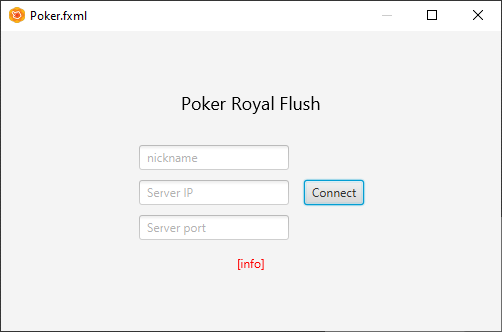
\includegraphics[width=70mm]{gui_start.png}
            \end{center}
            Ekran startowy włącza się po uruchomieniu programu. Służy on do połączenia się z serwerem.
            W odpowiednich polach wpisujemy:
            \begin{itemize}
                \item nickname - pseudonim pod jakim będą nas widzieć inni gracze (maksymalnie 10 znaków)
                \item Server IP - adres IP serwera do którego chcemy się połączyć
                \item Server port - numer port serwera do którego chcemy się połączyć
            \end{itemize}
            Przyciskiem \textbf{Connect} zainicjalizujemy próbę połączenia się z serwerem.\\
            Jeśli wpisane przez użytkownika dane będą niepoprawne, zostanie wyświetlony odpowiedni komunikat w miejscu \textbf{[info]}.
            
        \subsubsection{Ekran stołu gry}
            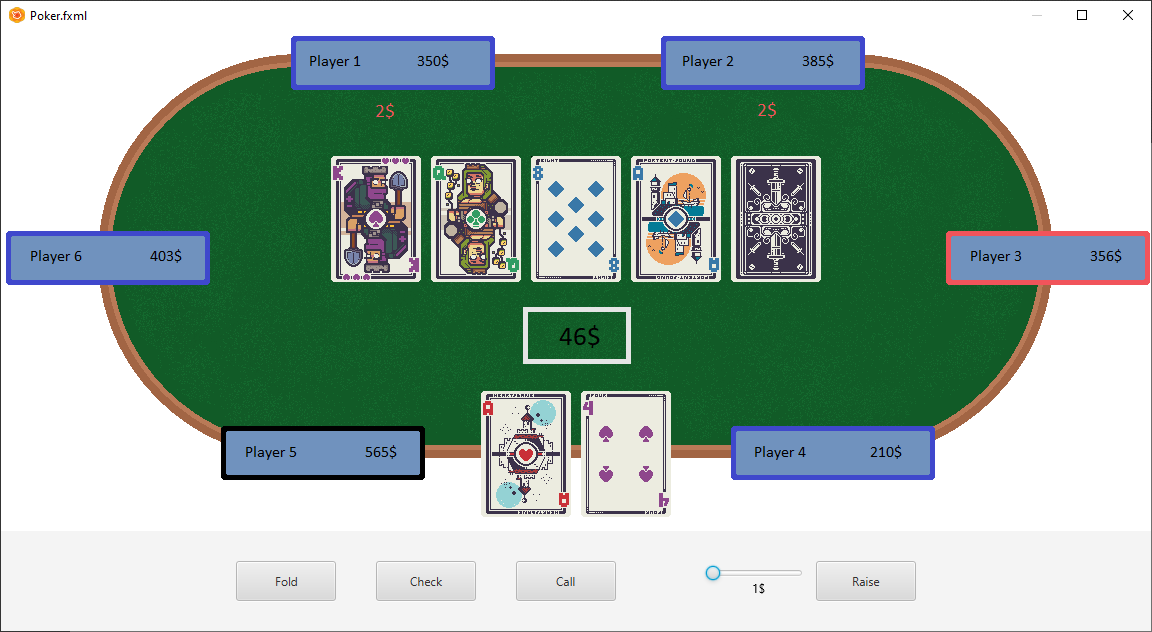
\includegraphics[width=\textwidth]{gui_table.png}
            Ekran stołu gry jest głównym ekranem aplikacji na którym, będzie rozgrywana gra.
            Składa się on z widoku stołu i menu wyboru ruchu.\\
            \\
            \textbf{Widok stołu}\\
            Niebieskie ramki zawierają informacje o danym graczu - pseudonimie i stanie konta.
            Obok ramek może pojawić się tekst, który informuje o tym ile dany gracz postawił pieniędzy w aktualnej turze. Ramka zapalona na:\\
            czerwono - informuje o tym, kogo jest teraz kolej,\\
            czarno - informuje o tym, czy gracz wykonał pas.\\
            Na środku stołu, po każdej turze, pokazują się kolejne karty wspólne.\\
            Pod kartami wspólnymi w białej ramce widoczna jest wartość puli w danej rundzie.\\
            Na dole widoku stołu znajdują się dwie karty, są to karty z ręki startowej gracza. Te karty widoczne są tylko dla gracza do którego one należą.\\
            \\
            \textbf{Menu wyboru ruchu}\\
            Menu wyboru ruchu składa się z 5 kontrolek - 4 przycisków i 1 suwaka. Kontrolki wyłączają się i włączają w zależności od: czy jest teraz kolej gracza, czy gracz może wykonać dany ruch w tym momencie.\\
            Kontrolki odpowiadają za:
            \begin{itemize}
                \item Przycisk \textbf{Fold} - pas; wycofanie się z rundy
                \item Przycisk \textbf{Check} - czekanie; gracz podczas swojej kolejki nie podejmuje żadnych działań
                \item Przycisk \textbf{Call} - sprawdzenie; postawić taką samą sumę pieniędzy ile wynosiło podbicie
                \item Suwak - służy do wybrania sumy pieniędzy o jaką gracz podbije pulę
                \item Przycisk \textbf{Raise} - podbicie; podbić pulę o taką sumę pieniędzy jaka została wybrana na suwaku
            \end{itemize}


\section{Testowanie}
    Poszczególne klasy programu zostaną przetestowane za pomocą testów jednostkowych. 
    Do tego posłuży narzędzie \textbf{JUnit 5}.
    Współpraca klas w programie oraz działanie graficznego interfejsu użytkownika zostanie przetestowane ręcznie w trakcie implementacji.
    Na koniec projektu, program zostanie jeszcze raz dogłębnie przetestowany pod kątem poprawnego działania wszystkich jego funkcji.

\end{document}
